\documentclass{jsreport}
\usepackage{graphicx, url, algorithm, algorithmic, float, booktabs, listings, color, pdfpages, amsmath, amssymb, latexsym, mathtools, ascmac, amsfonts, amsthm}
\lstset{
  basicstyle={\ttfamily},
  identifierstyle={\small},
  commentstyle={\smallitshape},
  keywordstyle={\small\bfseries},
  ndkeywordstyle={\small},
  stringstyle={\small\ttfamily},
  frame={tb},
  breaklines=true,
  columns=[l]{fullflexible},
  numbers=left,
  xrightmargin=0zw,
  xleftmargin=3zw,
  numberstyle={\scriptsize},
  stepnumber=1,
  numbersep=1zw,
  lineskip=-0.5ex
}
\usepackage[table,xcdraw]{xcolor}
\newtheorem{theo}{定理}[chapter]
\newtheorem{defi}{定義}[chapter]
\newtheorem{lemm}{補題}[chapter]
\newtheorem{prop}{命題}[chapter]
\newtheorem{coro}{系}[chapter]
\newcommand{\red}[1]{\textcolor{red}{#1}}
\newcommand{\blue}[1]{\textcolor{blue}{#1}}
\newcommand{\green}[1]{\textcolor{green}{#1}}
\renewcommand{\baselinestretch}{1.1}
\usepackage{mathrsfs}
\usepackage{bm}
\def\qed{\hfill $\Box$}
\usepackage{tikz}
\usetikzlibrary{intersections, calc, arrows}
\renewcommand\proofname{\bf 証明}

\begin{document}
\chapter{最適化問題の双対性}
本章では,非線形計画問題および凸計画問題における双対問題の性質と役割について述べる.
\section{ラグランジュ双対問題}
非線形計画問題において,すべての制約条件が不等式で与えられている場合を考える.つまり,
\begin{align}\label{eq:opt_nonl_f_true}
  \mathrm{minimize} \; \; &f(\bm{x}) \nonumber\\
  \mathrm{subject \; to} \; \; &g_i(\bm{x}) \leq 0, \; i = 1, 2, \ldots, m  \\
  &\bm{x} \in X \nonumber
\end{align}
を考える.集合$X \subseteq \mathbb{R}^n$は任意だが,以下の議論では$X = \mathbb{R}^n$あるいは$X = \mathbb{R}_{+}^n \, (= \{\bm{x} \in \mathbb{R}^n \, | \, \bm{x} \geq \bm{0}\})$を想定する.
この問題のLagrange関数は,ラグランジュ乗数ベクトル$\bm{u}$を用いて
\begin{equation}\label{eq:lag}
  L(\bm{x}, \bm{u}) = f(\bm{x}) + \bm{u}^{\mathrm{T}}g(\bm{x}), \; \bm{x} \in X, \bm{u} \in \mathbb{R}_{+}^m
\end{equation}
と定義される.

Lagrange関数と元の最適化問題の関係を調べるため,$x \in X$を固定し,$\bm{u}$に関する最大化問題
\begin{align}\label{eq:opt_lag}
  \mathrm{maximize} \; \; &L(\bm{x}, \bm{u}) \nonumber \\
  \mathrm{subject \; to} \; \; &\bm{u} \in \mathbb{R}_{+}^m
\end{align}
を導入し,この最大値($\infty$の場合もある)$\sup_{\bm{u} \geq \bm{0}} L(\bm{x}, \bm{u})$を$F(\bm{x})$と表す.
\begin{enumerate}
  \item $\exists i \; s.t. \; g_i(\bm{x}) > 0$のとき

  添字$i$に対応する$u_i$を大きくすれば問題(\ref{eq:opt_lag})の目的関数をいくらでも大きくすることができる.
  \item $g(\bm{x}) \leq \bm{0}$のとき

  $\bm{u}^{\mathrm{T}}g(\bm{x}) = 0$(例えば$\bm{u} = \bm{0}$)のとき,目的関数は最大値をとり,その値は$f(\bm{x})$である.
\end{enumerate}
よって,
\begin{equation}
  F(\bm{x}) = \begin{cases}
    f(\bm{x}), & g(\bm{x}) \leq \bm{0} \\
    \infty,        & \mathrm{otherwise}
\end{cases} \nonumber
\end{equation}
となる.したがって,元の問題(\ref{eq:opt_nonl_f_true})の最適値を$f^{*}$とすると,
\begin{equation}
  f^{*} = \inf_{\bm{x} \in X} F(\bm{x}) = \inf_{\bm{x} \in X} \sup_{\bm{u} \geq \bm{0}} L(\bm{x}, \bm{u}) \nonumber
\end{equation}
を得る.ただし,$g(\bm{x}) \leq \bm{0}$を満たす実行可能解$\bm{x}$がなければこの値は$\infty$である.場合によっては$-\infty$に発散することもある.

\begin{lemm}[inf-supとsup-inf]\label{lemm:infsup}
  Lagrange関数$L(\bm{x}, \bm{u})$は次の不等式を満たす\footnote{
  任意の$\tilde{\bm{x}} \in \mathbb{R}^n$に対して
  \begin{equation}
    \sup_{\bm{u} \geq \bm{0}} L(\tilde{\bm{x}}, \bm{u}) \geq \sup_{\bm{u} \geq \bm{0}} \inf_{\bm{x} \in X} L(\bm{x}, \bm{u}) \nonumber
  \end{equation}
  は明らか.左辺の$\inf_{\tilde{\bm{x}}}$をとっても不等号は成立することからこの補題は成立する.
  }.
  \begin{equation}
    \inf_{\bm{x} \in X} \sup_{\bm{u} \geq \bm{0}} L(\bm{x}, \bm{u}) \geq \sup_{\bm{u} \geq \bm{0}} \inf_{\bm{x} \in X} L(\bm{x}, \bm{u}) \nonumber
  \end{equation}
\end{lemm}

\paragraph{双対問題と弱双対定理}
Lagrange関数$L(\bm{x}, \bm{u})$において,$\bm{u} \in \mathbb{R}_{+}^m$を固定したのち,$\bm{x}$に関する次の最小化問題を考える.
\begin{align}\label{eq:opt_lag_x}
  \mathrm{minimize} \; \; &L(\bm{x}, \bm{u}) \nonumber \\
  \mathrm{subject \; to} \; \; &\bm{x} \in X
\end{align}
問題(\ref{eq:opt_lag_x})の最適値を$q(\bm{u})$と表すと,
\begin{equation}\label{eq:qu}
  q(\bm{u}) = \inf_{\bm{x} \in X} L(\bm{x}, \bm{u})
\end{equation}
である.$\bm{u}$の値によって$q(\bm{u}) = -\infty$も取りうる.補題\ref{lemm:infsup}より,
\begin{equation}\label{eq:infsup}
  \inf_{\bm{x} \in X} F(\bm{x}) = \inf_{\bm{x} \in X} \sup_{\bm{u} \geq \bm{0}} L(\bm{x}, \bm{u}) \geq
  \sup_{\bm{u} \geq \bm{0}} \inf_{\bm{x} \in X} L(\bm{x},\bm{u}) = \sup_{\bm{u}
  \geq \bm{0}} q(\bm{u})
\end{equation}
を得る.この最後の問題を元の最適化問題(\ref{eq:opt_nonl_f_true})のラグランジュ双対問題(Lagrangian dual problem)と呼ぶ.つまり,次の問題である.
\begin{align}\label{eq:lag_dual}
  \mathrm{maximize} \; \; &q(\bm{u}) \nonumber \\
  \mathrm{subject \; to} \; \; &\bm{u} \in \mathbb{R}_{+}^m
\end{align}


\begin{theo}[弱双対定理(weak duality)]\label{theo:weak_dual}
  主問題(\ref{eq:opt_nonl_f_true})の最適値を$f^{*}$,双対問題(\ref{eq:lag_dual})の最適値を$q^{*}$とすると,次の関係が成立する\footnote{
  $f^{*} = \inf_{\bm{x} \in X} F(\bm{x})$および
  $q^{*} = \sup_{\bm{u} \geq \bm{0}} q(\bm{u})$より.
  }.
  \begin{equation}
    f^{*} \geq q^{*} \nonumber
  \end{equation}
\end{theo}

次の最適化問題を例に考える.
\begin{align}
  \mathrm{minimize} \; \; &f(\bm{x}) = 2x_1^2 + x_1x_2 + x_2^2 - 5x_1 - 3x_2 + 4 \nonumber\\
  \mathrm{subject \; to} \; \; &g_1(\bm{x}) = x_1 + x_2 -1 \leq 0 \nonumber \\
  &\bm{x} \in \mathbb{R}^2 \nonumber
\end{align}

目的関数および制約式の勾配ベクトルは,
\begin{align}
  \nabla f(\bm{x}) &= (4x_1 + x_2 - 5, x_1 + 2x_2 - 3)^{\mathrm{T}} \nonumber \\
  \nabla g_1(\bm{x}) &= (1, 1)^{\mathrm{T}} \nonumber
\end{align}
である.よって,$f$の停留点は,$(1, 1)$である.また,$f$のヘッセ行列は,
\begin{equation}
  \nabla^2 f(\bm{x}) = \left(
  \begin{array}{cc}
    4 & 1 \\
    1 & 2
  \end{array}
  \right) \nonumber
\end{equation}
から,固有値は$\lambda_1 = 3 + \sqrt{2}, \lambda_2 = 3 - \sqrt{2}$であり,固有値$\lambda_1, \lambda_2$に属する固有ベクトルはそれぞれ$\bm{v}_1 = (1, \sqrt{2} - 1)^{\mathrm{T}}, \bm{v}_2 = (1, -\sqrt{2} - 1)^{\mathrm{T}}$である.
この問題の実行可能領域および$f$の等高線を図\ref{fig:feasible_ex}に示す.
\begin{figure}[tb]
  \centering
  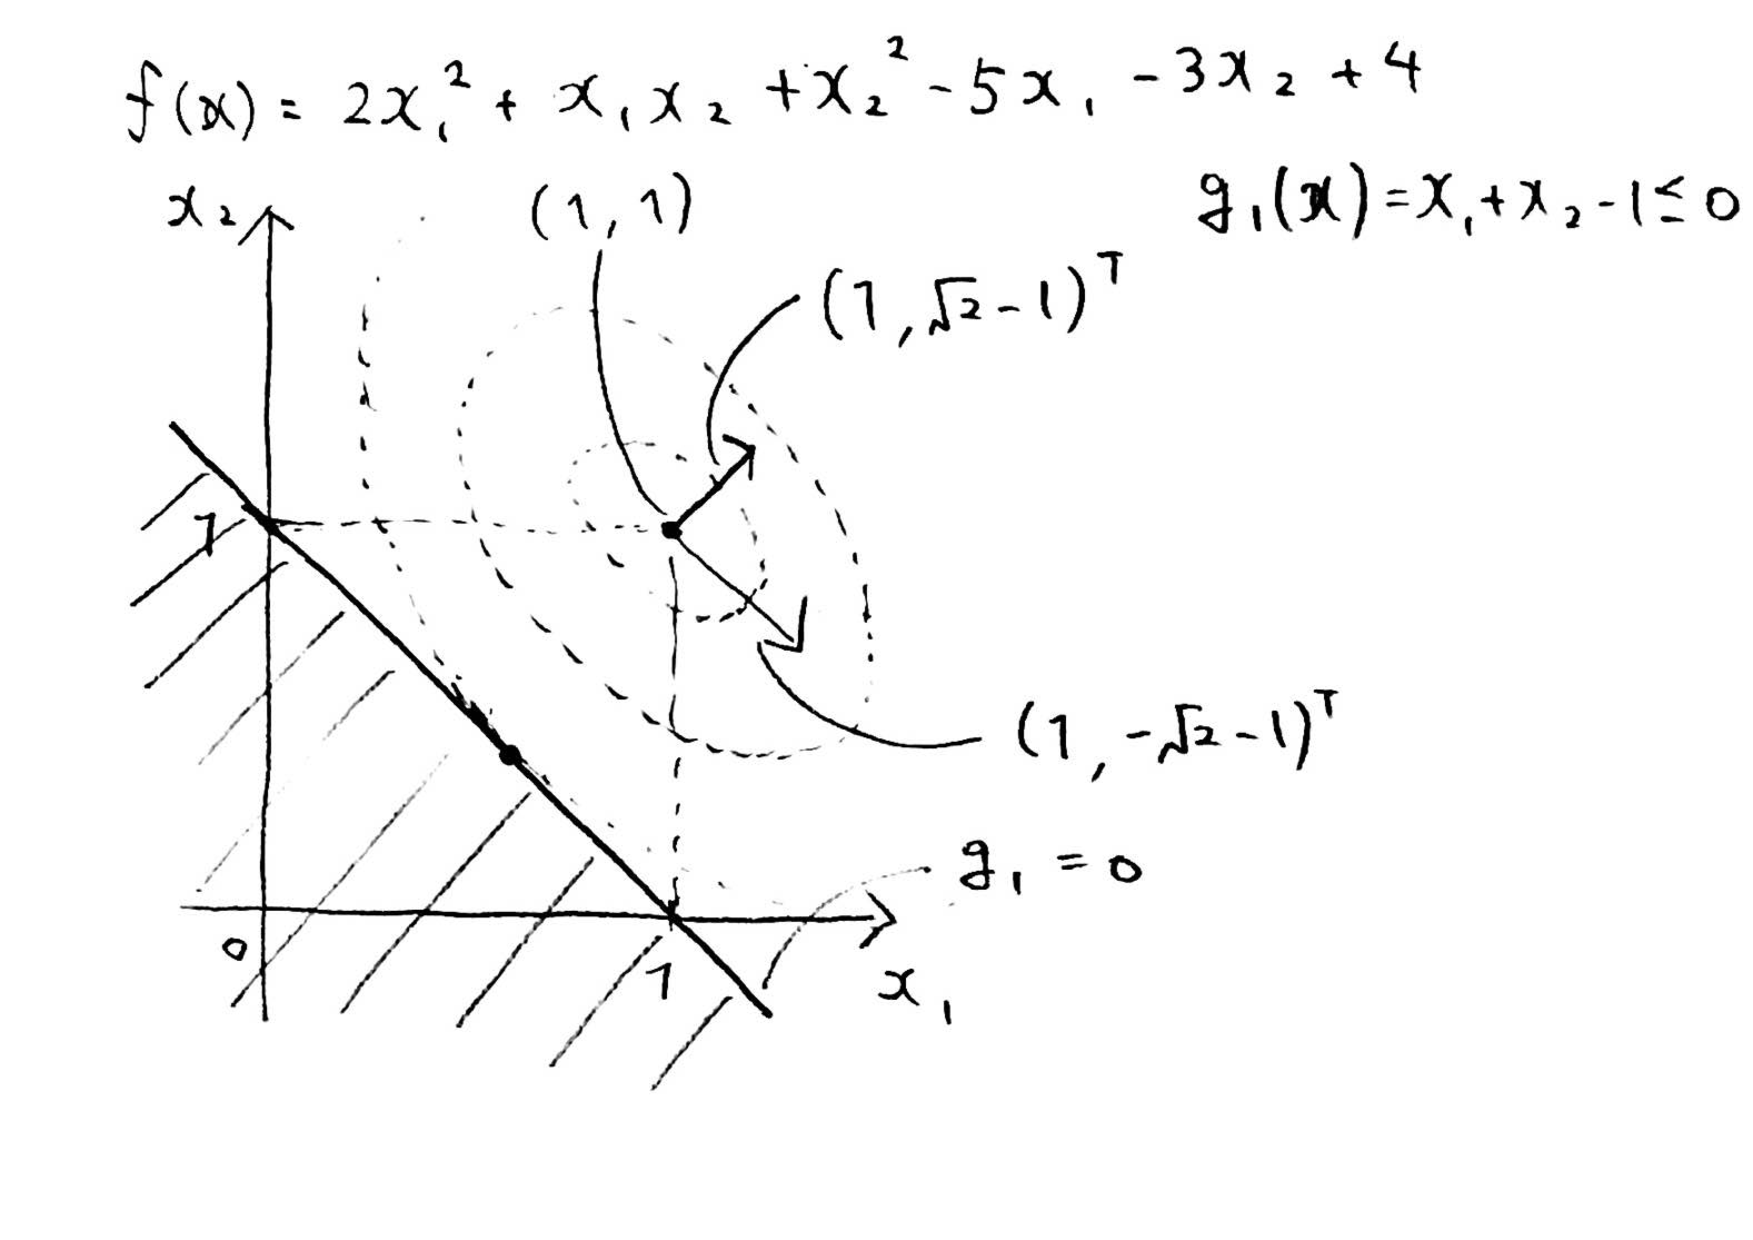
\includegraphics[clip, width=7cm]{../figure/KKT_3.pdf}
  \caption{実行可能領域と$f$の等高線}
  \label{fig:feasible_ex}
\end{figure}

$g_1(\bm{x})$は有効制約であると考えられる.よって,KKT条件は
\begin{align}
  &\left(
  \begin{array}{c}
    4x_1 + x_2 - 5 \\
    x_1 + 2x_2 - 3
  \end{array}
  \right) + u\left(
  \begin{array}{c}
    1 \\
    1
  \end{array}
  \right) = \left(
  \begin{array}{c}
    0 \\
    0
  \end{array}
  \right) \nonumber \\
  &x_1 + x_2 - 1 = 0 \nonumber
\end{align}
より,
\begin{equation}
  (\bar{x}_1, \bar{x}_2, u) = \left(\frac{3}{4}, \frac{1}{4}, \frac{7}{4} \right) \nonumber
\end{equation}
を得る.容易にわかるようにこれは最適解であり,最適値は
\begin{equation}
  f^{*} = \frac{7}{8} \nonumber
\end{equation}
である.

次に,この問題の双対問題を考える.Lagrange関数は,
\begin{equation}
  L(\bm{x}, u) = 2x_1^2 + x_1x_2 + x_2^2 + (u - 5)x_1 + (u - 3)x_2 + 4 - u \nonumber
\end{equation}
である.$u$を固定して$q(u)$を求めるため,停留点条件
\begin{equation}
  \nabla_{\bm{x}} L(\bm{x}, u) = \left(
  \begin{array}{c}
    4x_1 + x_2 + u - 5 \\
    x_1 + 2x_2 + u - 3
  \end{array}
  \right) = \left(
  \begin{array}{c}
    0 \\
    0
  \end{array}
  \right) \nonumber
\end{equation}
を解くと,
\begin{equation}
  x_1 = 1 - \frac{3}{7} u, \; x_2 = 1 - \frac{1}{7} u \nonumber
\end{equation}
を得る.この結果を$L(\bm{x}, u)$に代入して整理すると,
\begin{equation}
  q(u) = -\frac{2}{7} u^2 + u = - \frac{2}{7}\left(u - \frac{7}{4}\right)^2 + \frac{7}{8} \nonumber
\end{equation}
となる.したがって,双対問題は
\begin{align}
  \mathrm{maximize} \; \; &-\frac{2}{7} u^2 + u \nonumber\\
  \mathrm{subject \; to} \; \; &u \in \mathbb{R}_{+} \nonumber
\end{align}
と書ける.この問題の最適解は$u = 7/4$であり,最適値は
\begin{equation}
  q^{*} = \frac{7}{8} \nonumber
\end{equation}
である.以上をまとめ,$f^{*} = q^{*}$の成立が判明した.\qed

\paragraph{鞍点と最適性}
Lagrange関数$L(\bm{x}, \bm{u})$に対し,次の条件を満たす$\bm{x}^{*} \in X, \, \bm{u}^{*} \in \mathbb{R}_{+}^{m}$が存在するならば,$(\bm{x}^{*}, \bm{u}^{*})$を$L$の鞍点(saddle point)という.
\begin{equation}\label{eq:saddle}
  L(\bm{x}, \bm{u}^{*}) \geq L(\bm{x}^{*}, \bm{u}^{*}) \geq L(\bm{x}^{*}, \bm{u}), \; \forall \bm{x} \in X, \, \forall \bm{u} \in \mathbb{R}_{+}^{m}
\end{equation}

\begin{coro}
  主問題(\ref{eq:opt_nonl_f_true})と双対問題(\ref{eq:lag_dual})に対し,以下の条件はそれぞれ$\bm{x}^{*} \in X$が主問題の,$\bm{u}^{*}$が双対問題の最適解であるための十分条件である.
  \begin{enumerate}
    \item $\bm{x}^{*}$は主問題の実行可能解,$\bm{u}^{*}$は双対問題の実行可能解であり,さらに$f(\bm{x}^{*}) = q(\bm{u}^{*})$を満たす.
    \item $(\bm{x}^{*}, \bm{u}^{*})$はLagrange関数$L(\bm{x}, \bm{u})$の鞍点である.
  \end{enumerate}
\end{coro}

\paragraph{等式制約がある場合の双対問題}

\begin{align}\label{eq:opt_nonl_eq_dual}
  \mathrm{minimize} \; \; &f(\bm{x}) \nonumber\\
  \mathrm{subject \; to} \; \; &g_i(\bm{x}) \leq 0, \; i = 1, 2, \ldots, l \nonumber \\
  &g_i(\bm{x}) = 0, \; i = l+1, \ldots, m \\
  &\bm{x} \in X \nonumber
\end{align}

等式条件は,
\begin{equation}
  g_i(\bm{x}) \leq 0, \; -g_i(\bm{x}) \leq 0, \; i = l + 1, \ldots, m \nonumber
\end{equation}
と不等式の対で表し,対応するラグランジュ乗数をそれぞれ$u_i^{+}, \, u_i^{-}$と記すと,Lこの問題のLagrange関数は
\begin{equation}\label{eq:lag_eq}
  L(\bm{x}, \bm{u}) = f(\bm{x}) + \sum_{i = 1}^l u_i g_i(\bm{x}) + \sum_{i = l + 1}^{m}(u_i^{+} - u_i^{-})g_i(x)
\end{equation}
である.ただし,
$u_i \geq 0, i = 1, 2, \ldots, l, \; u_i^{+}, u_i^{-} \geq 0, i = l + 1, \ldots, m$
であるが,
\begin{equation}
  u_i = u_i^{+} - u_i^{-}, \; i = l + 1, \ldots, m
\end{equation}
とおくと,$u_i$は正負どちらの値もとることができて符号制約はなくなる.この$u_i$を用いると,LLこの問題のLagrange関数は
\begin{equation}
  L(\bm{x}, \bm{u}) = f(\bm{x}) + \sum_{i = 1}^m u_i g_i(\bm{x}) \nonumber
\end{equation}
ただし,
\begin{align}\label{eq:lag_u}
  &u_i \geq 0, \; i = 1, 2, \ldots, l \nonumber \\
  &u_i \, : \, 符号制限なし, \; i = l + 1, \ldots, m
\end{align}
となる.つまり,等式条件に対するラグランジュ乗数の符号制限がなくなる点だけが異なる.

この$L(\bm{x}, \bm{u})$から双対問題に至るまでは,不等式制約のみの議論をほぼそのまま適用することができる.得られる双対問題は,
\begin{align}\label{eq:dual_eq}
  \mathrm{maximize} \; \; &q(\bm{u}) \nonumber \\
  \mathrm{subject \; to} \; \; &\bm{u} \in \mathbb{R}^m \\
  &u_i \geq 0, \; i = 1, 2, \ldots, l \nonumber
\end{align}
である.弱双対定理\ref{theo:weak_dual}もそのまま成立する.

\section{凸計画問題の双対定理}
主問題として
\begin{align}\label{eq:opt_nonl_f_convex}
  \mathrm{minimize} \; \; &f(\bm{x}) \nonumber\\
  \mathrm{subject \; to} \; \; &g_i(\bm{x}) \leq 0, \; i = 1, 2, \ldots, m  \\
  &\bm{x} \in \mathbb{R}^n \nonumber
\end{align}
を考える.ただし,$f(\bm{x})$および$g_i(\bm{x}), \, i = 1, 2, \ldots, m$はすべて凸関数である.さらに,実行可能領域は内点$\bm{x}^{\prime} \in \mathbb{R}^n$を持つ(Slaterの制約想定).
\begin{equation}\label{eq:slater}
  g_i(\bm{x}^{\prime}) < 0, \; i = 1, 2, \ldots, m
\end{equation}
このとき,次の定理が成立する.
\begin{theo}[凸計画問題の双対定理]\label{theo:dual_convex}
  凸計画問題(\ref{eq:opt_nonl_f_convex})がSlaterの制約想定(\ref{eq:slater})を満たすと仮定し,最適値を$f^{*}$,その双対問題(\ref{eq:lag_dual})の最適値を$q^{*}$と記す.このとき,$f^{*} = q^{*}$が成立する.
\end{theo}



\end{document}
